\chapter{Clustering Algorithm and Application}
\label{chapter:clustering}

The objective of classification is to find assignments between data points and categories. For some applications this can be done by taking correctly labelled data and comparing a new data point to the data points in different categories to see which category best fits. One such algorithm is k-nearest-neighbour. In our context the issue with this approach is that the data is only labelled as to which experiment it came from, e.g. positive control in human cells, negative control in mouse cells. However, as noted before not all cells from these experiments behaved as we expected them to, e.g. some cells activated in the negative control or did not activate in the positive control. Therefore, we choose to use a clustering algorithm which does not have the need for classified training data.

\section{Gaussian Mixture Model}
\label{sec:gaussian_mixture_model}

This section follows the article Gaussian Mixture Model by Reynolds~\cite{reynolds2009}.

Often gathered observations are distributed as a normal distribution. These distributions have a density function
\begin{align*}
	g(x|\mu, \Sigma) = \frac{1}{(2\pi)^{D/2} |\Sigma|^{1/2}} exp\left( - \frac{1}{2} (x-\mu)^T \Sigma^{-1} (x-\mu) \right)
\end{align*}
with parameters $D$ called the dimension, $\mu$ called the mean vector and $\Sigma$ called the covariance matrix.

As we are concerned with clustering data points we expect the observed data points from different clusters to have different parameters in the normal distribution they come from. Assuming we have $n$ different data sources gives us normal distributions $g_i(x|\mu_i, \Sigma_i)$ where $i=1, ..., n$. Additionally, we might have more data points being generated from some normal distributions while less from others. We can express this using another weight parameter $w_i$ with $i=1, ..., n$. To normalize the weights we set the constraint $\sum w_i = 1$.

The distribution describing the entire dataset now can be described with the distribution
\begin{align}
	\label{eq:sum_of_normal}
	p(x) = \sum_{i=1}^{n} w_i g(x|\mu_i, \Sigma_i).
\end{align}

Gaussian Mixture Model is a method to retrieve these parameters $w_i$, $\mu_i$ and $\Sigma_i$ for some $D$ dimensional data points generated from $n$ normal distributions.

From these parameters it is easy to cluster the data as we know where data points from the different clusters are expected to lie.

From equation~\ref{eq:sum_of_normal} we expect every $\Sigma_i$ to be independent of each other. In the context of Gaussian Mixture Models this is called having a full covariance matrix. However, we can eliminate some of the variables in the covariance matrix if we choose a diagonal covariance matrix. Additionally, we might specify to use the same covariance matrix for all $i$, which is called tied in this context.

Choosing a full covariance matrix is not necessary even if the data is expected to have statistically independent features, as the overall density is compromised from multiple normal distributions with diagonal $\Sigma_i$. This enables us to model correlations between features.

The question now is how we can derive the parameters $w_i, \mu_i$ and $\Sigma_i$. We choose the approach which chooses the parameters where the likelihood that the data was generated by these parameters is maximal. This is known as maximum likelihood estimation. The likelihood can be expressed as

\begin{align*}
	L(w_i, \mu_i, \Sigma_i|X) = p(X|w_i, \mu_i, \Sigma_i) = \prod_{t=1}^n p(x_t|w_i, \mu_i, \Sigma_i)
\end{align*}

with $X = (x_1, ..., x_n)$ being the recorded data. As $L(w_i, \mu_i, \Sigma_i|X)$ is non-linear in the parameters deriving the maximum is not trivial. Instead, we use an iterative approach which approaches the solution. Define $\lambda = (w_i, \mu_i, \Sigma_i)$. Simplifying to a diagonal covariance matrix gives us the iterative algorithm where we define the successor values $\bar{.}$ as

\begin{align*}
	Pr(i | x_t, \lambda) := \frac{w_i g(x_t | \mu_i, \Sigma_i)}{\sum_{k=1}^{n} w_k g(x_t | \mu_k, \Sigma_k)}\\
	\bar{w}_i := \frac{1}{n} \sum_{t=1}^{n} Pr(i | x_t, \lambda)\\
	\bar{\mu}_i := \frac{\sum_{t=1}^{n} Pr(i | x_t, \lambda) x_t}{\sum_{t=1}^{n} Pr(i | x_t, \lambda)}\\
	\bar{\sigma}_i^2 := \frac{\sum_{t=1}^{n} Pr(i | x_t, \lambda) x_t^2}{\sum_{t=1}^{n} Pr(i | x_t, \lambda)} - \bar{\mu}_i^2.
\end{align*}

for $w_i$, $\mu_i$ and $\sigma_i^2$ respectively. One can show that with this iteration rule we have $p(X|\bar{\lambda}) \geq p(X|\lambda)$. The value $Pr(i|x_t, \lambda)$ is known as the a posteriori probability for the i-th component.

From the parameters $w_i, \mu_i$ and $\sigma_i^2$ we can get the probability of a data point belonging to the $i$-th cluster. This data point can be either one of the ones used to get the parameters or a new one.

\section{KMeans}

We want to explore a second clustering algorithm. Like Gaussian Mixture Model this method assigns data points to clusters after having been trained with unlabelled data.

Once again we assume to have $k$ different data sources from where the data stems. As the data from every of these resulting clusters will be close to each other, we have that the variance within the cluster is relatively small compared to the variance of data points from different clusters.

The variance of data points $(x_n)_{n=1, ..., m}$ is calculated as
\begin{align*}
	Var((x_n)_{n=1, ..., m}) = \frac{1}{m} \sum_{n=1}^{m} ||x_n - \mu||^2, && \text{where} && \mu = \frac{1}{m} \sum_{n=1}^{m} x_n.
\end{align*}

We can therefore formulate the problem as a minimization problem. Using $k$ clusters $S_1, ..., S_k$, with $|S_l|$ data points in each, we want to minimize the sum of variants
\begin{align*}
	\sum_{l=1}^{k} \sum_{x \in S_l} ||x - \mu_l||^2 = \sum_{l=1}^{k} |S_l| Var(S_l).
\end{align*}

We want to show that this is equivalent to minimizing
\begin{align*}
	\sum_{l=1}^{k} \frac{1}{|S_l|} \sum_{x, y \in S_l} ||x-y||^2.
\end{align*}

This follows from the equality

\begin{align*}
	\frac{1}{|S_l|} \sum_{x, y \in S_l} ||x-y||^2 =\\
	\frac{1}{|S_l|} \sum_{x, y \in S_l} ||x||^2 - 2||x||\cdot||y|| + ||y||^2 =\\
	\frac{1}{|S_l|} (|S_l| \sum_{x\in S_l} ||x||^2 - 2\sum_{x, y \in S_l}||x|| ||y|| + |S_l| \sum_{y \in S_l}||y||^2) =\\
	\frac{1}{|S_l|} (|S_l|^2 E(S_l^2) - 2(\sum_{x\in S_l}||x||)(\sum_{y \in S_l}||y||) + |S_l|^2 E(S_l^2)) =\\
	2|S_l| E(S_l^2) - 2|S_l| E(S_l)^2 =\\
	2 |S_l| Var(S_l).
\end{align*}

Minimizing is hard, but is typically solved by the approximation using the following algorithm consisting of two steps.

\begin{itemize}
	\item Assign all data points to clusters $S_1, ..., S_k$, by choosing the cluster $S_l$ with the closest mean $\mu_l$.
	\item Update the means $\mu_l$ by calculating them as the mean of the data points assigned to $S_l$.
\end{itemize}

We formulate this mathematically as the successor $\hat{S}_l$ and $\mu_l$ of $S_l$ and $\mu_l$ respectively being

\begin{align*}
	\hat{S}_l := \{x: ||x-\mu_l|| \leq ||x-\mu_j|| \forall j \in \{1, ..., k\} \} &&
	\hat{\mu}_l := \frac{1}{|\hat{S}_l|} \sum_{x \in \hat{S}_l} x.
\end{align*}

From the definition of $\hat{S}_l$ and $\hat{\mu}_i$ it follows that

\begin{align*}
	\sum_{l=1}^{k} \frac{1}{|\hat{S}_l|} \sum_{x, y \in \hat{S}_l} ||x-y||^2 \leq \sum_{l=1}^{k} \frac{1}{|S_l|} \sum_{x, y \in S_l} ||x-y||^2.
\end{align*}

The convergence of the algorithm towards a minimum seems likely. The choice of initial values can have a big impact on the result.

\section{Implementation of the Clustering Algorithm}

Python offers an implementation of Gaussian Mixture Model and KMeans with the sklearn package. The function with parameters relevant to us is

\noindent
\texttt{sklearn.mixture.GaussianMixture(n\_components, covariance\_type, n\_init)} and

\noindent
\texttt{sklearn.cluster.KMeans(n\_clusters, n\_init)}. The number of components

\noindent
\texttt{n\_components} or \texttt{n\_clusters} can be any positive integer. The \texttt{covariance\_type} can be one of \texttt{‘full’, ‘tied’, ‘diag’} or \texttt{‘spherical’} and describes what type of covariance matrix is used. The parameter \texttt{n\_init} lets the algorithm run multiple times and returns the parameters of the best clustering achieved.

As the input of the clustering we use data points of the form \texttt{[a, u, d, k1, k2, w1, w2]}, where \texttt{a, u, ..., w2} are the parameters of the approximation from chapter~\ref{chapter:approximating}. As our goal is to separate data points from the four data sets mouse cells and human cells each with a negative and a positive control, we use all particles as input. The pseudo code below describes the steps performed to reach a clustering of the data.

\begin{algorithm}[H] \label{alg:separate}
	\SetAlgoLined
	\DontPrintSemicolon
	\LinesNumbered
	\SetKwInOut{Input}{input}
	\SetKwInOut{Output}{output}
	\caption{Separate}
	
	\Input{parameters of the approximations of all particles in all data sets}
	\Output{assignments to different clusters for each particle, parameters specifying each cluster}
	
	\BlankLine
	\Begin{
		initialize Gaussian Mixture or KMeans by specifying the number of components and \texttt{covariance\_type} for Gaussian Mixture\;
		apply clustering method to matrix of all parameters of the approximations of all particle data sets\;
		assign particles to clusters according to clustering results\;
		compare asignments from clustering to those of the data set the data stems from\;
		\Return{assignments to clusters, parameters specifying every cluster}
	}
\end{algorithm}
\vspace{1cm}

When comparing different covariance types in the Gaussian Mixture we see that using \texttt{‘diag’} we have the lowest error rate. The details are shown in table~\ref{tab:covariance_type_comparison}. Why reducing the number of parameters in the covariance matrix can yield better results is described in section~\ref{sec:gaussian_mixture_model}.

\begin{table}[h!]
	\centering
	\begin{tabular}{|c|c|}
		\hline
		\texttt{full}: $13.23\%$ & \texttt{tied}: $12.7\%$ \\
		\hline
		\texttt{diag}: $7.17\%$ & \texttt{spherical}: $31.52\%$ \\
		\hline
	\end{tabular}
	\caption{Error as a percentage of particles being assigned the wrong component.}
	\label{tab:covariance_type_comparison}
\end{table}

Using a diagonal covariance matrix we can now try to separate the data sets and visualize the results. As the data is 7 dimensional we show lower dimensional representations of the data both as it is assigned according to the data set it stems from as well as the assignment from algorithm~\ref{alg:separate}.

Choosing good axis for visualizing high dimensional data is tricky. One approach for minimizing the data lost by the lower dimensional representation is called Principal Component Analysis. Axis are specifically chosen to maximize variance along those axes, which we assume corresponds to information displayed along the axis. The drawback is that the new axis can are more difficult to intuitively understand. The results can be seen in figure~\ref{fig:vis_output_seperate_human_gaussian_mixture}, figure~\ref{fig:vis_output_seperate_human_kmeans}, figure~\ref{fig:vis_output_seperate_mouse_gaussian_mixture} and~\ref{fig:vis_output_seperate_mouse_kmeans}.

\begin{figure}
	\centering
	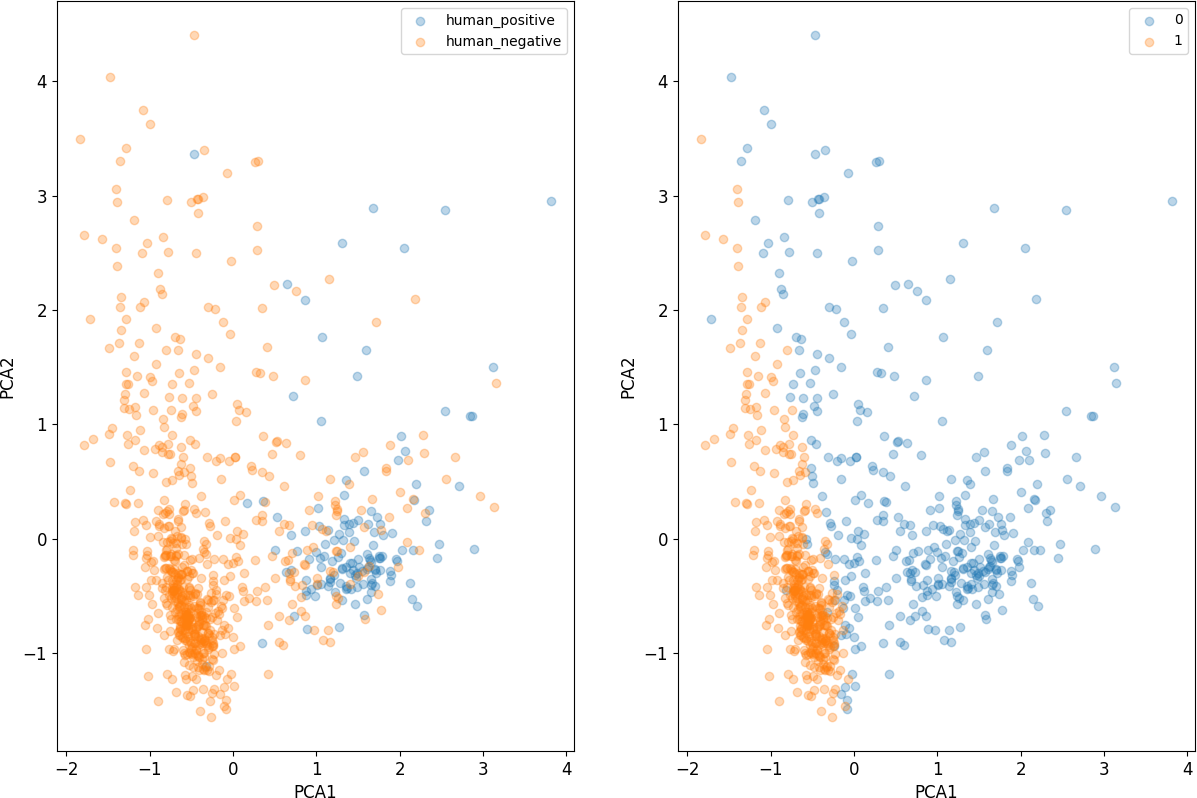
\includegraphics[width=\textwidth]{fig/separate_human_gaussian_mixture}
	
	\caption{Visualization of the clustered data points. The left image depicts the clustering according to positive and negative control on humans t cells. The right image shows the clustering according to Gaussian Mixture.}
	\label{fig:vis_output_seperate_human_gaussian_mixture}
\end{figure}
	
	
\begin{figure}
	\centering
	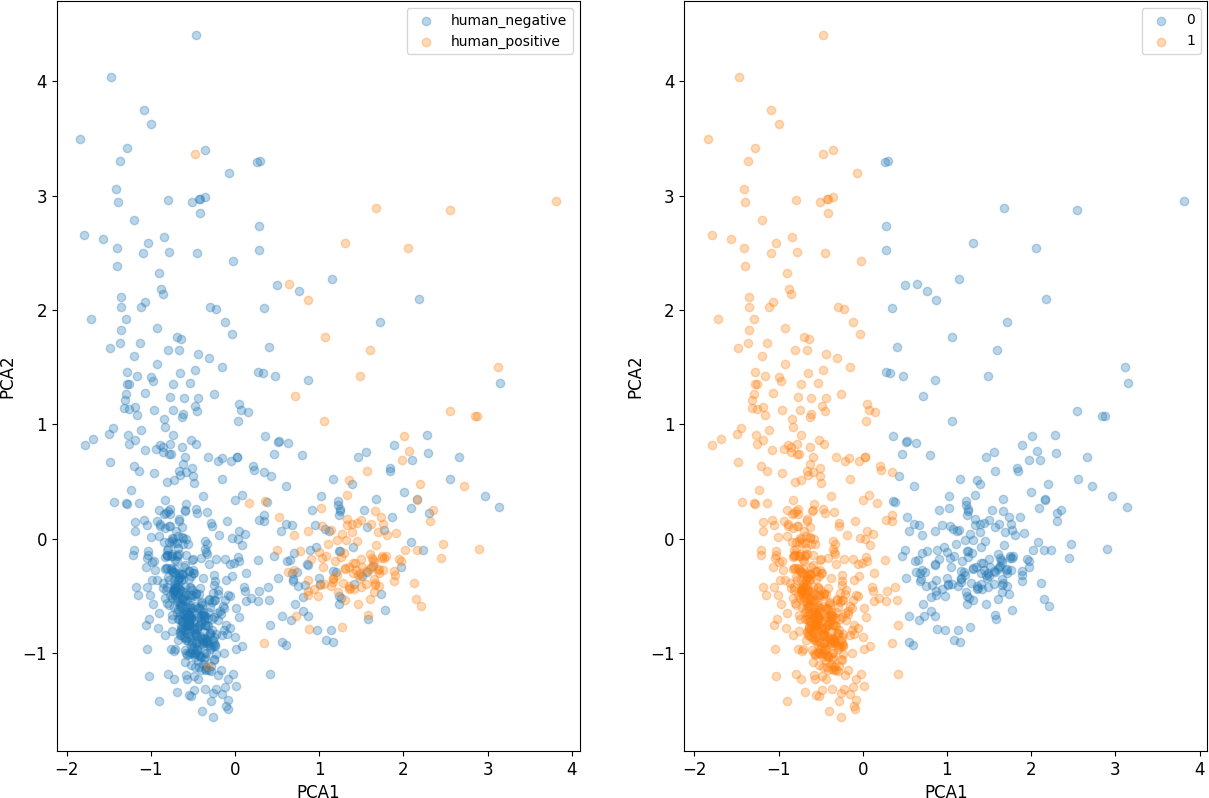
\includegraphics[width=\textwidth]{fig/separate_human_kmeans}
	
	\caption{Visualization of the clustered data points. The left image depicts the clustering according to positive and negative control on humans t cells. The right image shows the clustering according to KMeans.}
	\label{fig:vis_output_seperate_human_kmeans}
\end{figure}

\begin{figure}
	\centering
	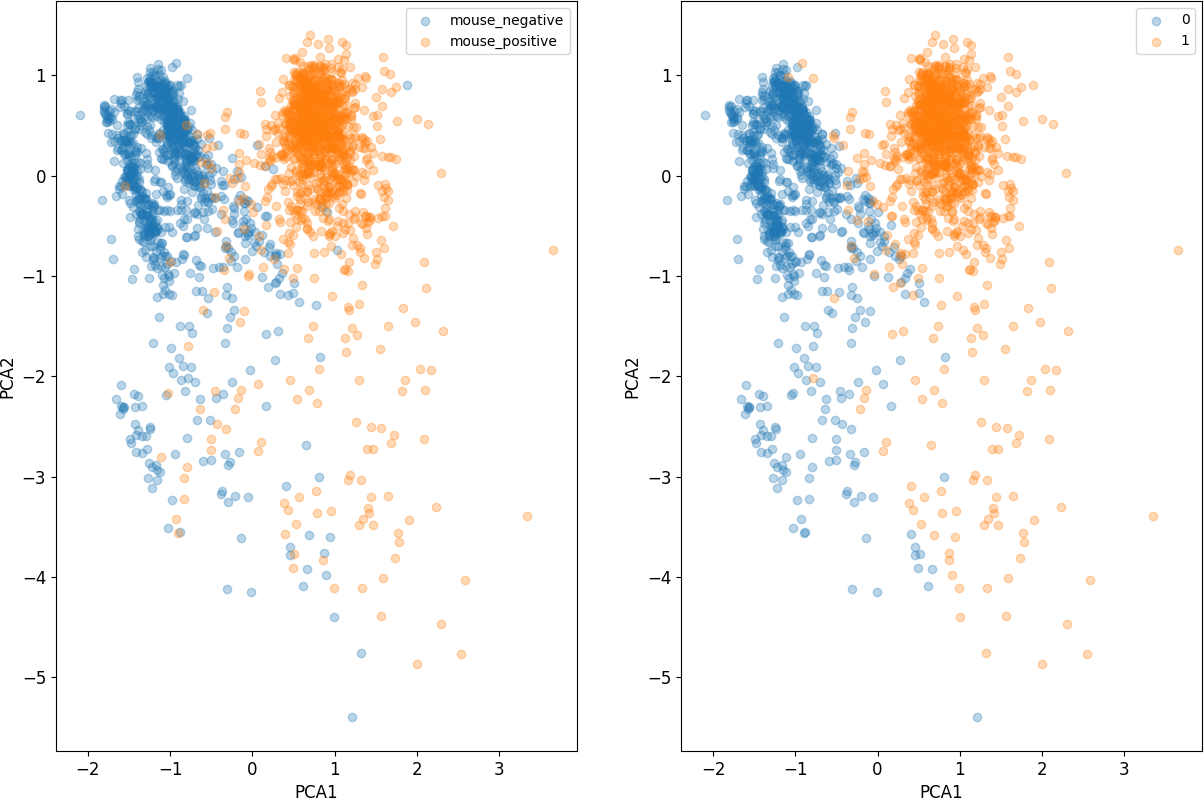
\includegraphics[width=\textwidth]{fig/separate_mouse_gaussian_mixture}
	
	\caption{Visualization of the clustered data points. The left image depicts the clustering according to positive and negative control on mouse t cells. The right image shows the clustering according to Gaussian Mixture.}
	\label{fig:vis_output_seperate_mouse_gaussian_mixture}
\end{figure}


\begin{figure}
	\centering
	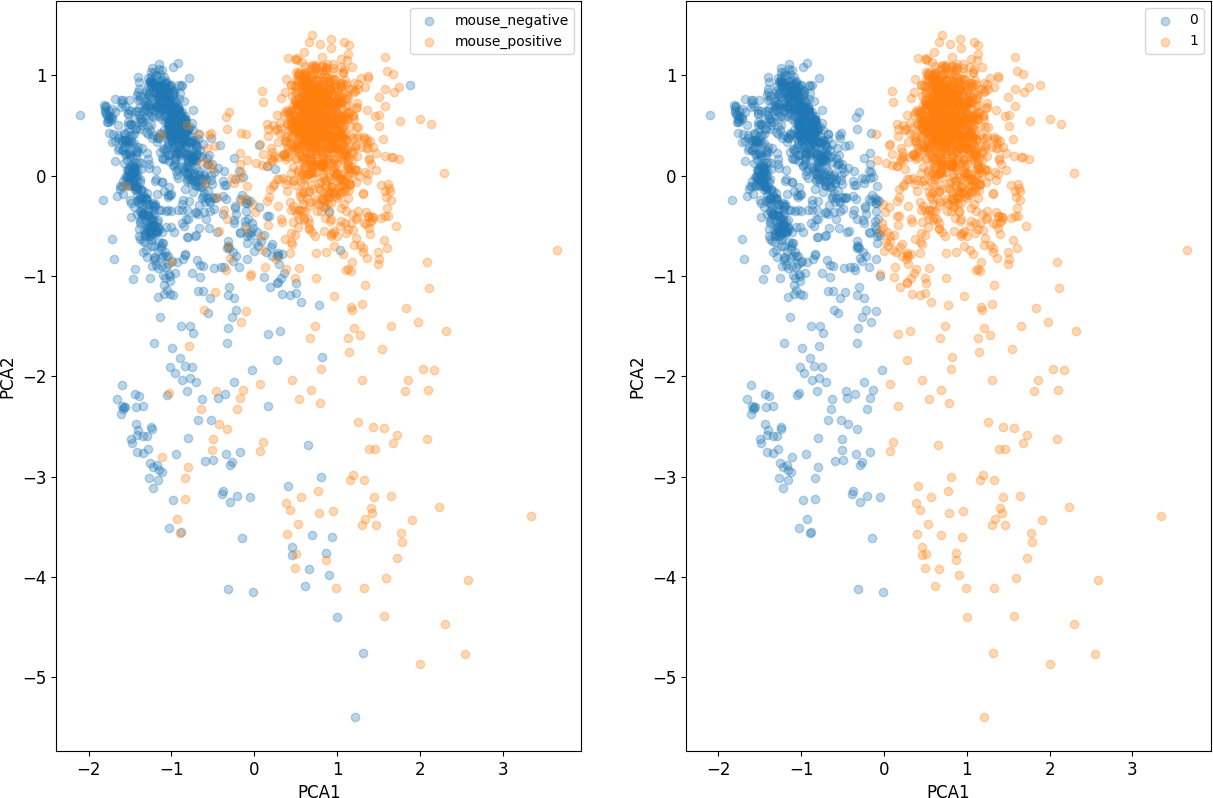
\includegraphics[width=\textwidth]{fig/separate_mouse_kmeans}
	
	\caption{Visualization of the clustered data points. The left image depicts the clustering according to positive and negative control on mouse t cells. The right image shows the clustering according to KMeans.}
	\label{fig:vis_output_seperate_mouse_kmeans}
\end{figure}

By comparing which data points are from which data set and where they were assigned by the clustering method we can find an assignment between the two.

The relevant information derived from the Gaussian Mixture clustering is the means and covariances of the four components. For KMeans clustering the means of the components are relevant. In both cases we can decide which cluster a new data point belongs to from this information. A use case might be to find percentages of activated cells in an experiment. Distinguishing between mouse and human cells does not have a clear use case. When specifying \texttt{n\_components=2} we assume to have a cluster for activated and a second for unactivated cells.

In comparison, to the approach focusing on outlier detection in section~\ref{sec:analysis_of_approximation} we now have an approach that is not only not dependent on parameters specified by a user, but can also be applied to a greater set of problems. A proposed way of answering the research questions from chapter~\ref{chapter:introduction} using these methods is described in chapter~\ref{chapter:results}.